\chapter{Inference for population proportions}
\label{c_probs}

\section{Introduction}
\label{s_probs_intro}

In this chapter we still consider statistical analyses which involve
only discrete, categorical variables. In fact, we now focus on the
simplest case of all, that of \textbf{dichotomous} (binary) variables
which have only two possible values. Four examples which will be used
for illustration throughout this chapter are introduced in Section
\ref{s_probs_examples}. In the first two of them we consider a
binary variable in a single population, while in the last two examples
the question of interest involves a comparison of the distributions of
the variable between two populations (\emph{groups}).

The data for such analyses can be summarised in simple tables, the
one-group case with a one-way table of two cells, and the two-group case
with a $2\times 2$ contingency table. Here, however, we formulate the
questions of interest slightly differently, with primary emphasis on the
\emph{probability} of one of the two values of the variable of interest. In the
one-group case the questions of interest are then about the population
value of a single probability, and in the two-group case about the
comparison of the values of this probability between the two groups.

While we describe specific methods of inference for these cases, we also
use them to introduce some further general elements of statistical
inference:
\begin{itemize}
\item
Population \textbf{parameters} of probability distributions.
\item
\textbf{Point estimation} of population parameters.
\item
Hypotheses anout the parameters, and significance tests
for them.
\item
\textbf{Confidence intervals} for population parameters.
\end{itemize}

The comparisons in the two-group analyses again address questions about
associations, now between the group and the dichotomous variable of
interest. Here it will be useful to employ the terminology
introduced in Section \ref{ss_intro_def_assoc}, which distinguishes
between the \textbf{explanatory variable} and the \textbf{response
variable} in the association. Following a common convention, we will
denote the explanatory variable by $X$ and the response variable by $Y$.
In the two-group cases of this chapter, $X$ will be the group (which is
itself also binary) and $Y$ the binary variable whose probabilities we
are interested in. We will use $Y$ to denote this binary variable also
in the one-group examples.


\section{Examples}
\label{s_probs_examples}

The following four examples will be discussed in this chapter. Examples
5.1 and 5.2 concern only one group, while in Examples 5.3
and 5.4 two groups are to be compared. Table \ref{t_probex} shows basic
sample statistics for the examples, together with the results of the
significance tests and confidence intervals described later.

\underline{\textbf{Example 5.1}}: \textbf{An EU referendum}

A referendum about joining the European Union was held in Finland on the
16th of October, 1994. Suppose that in an opinion poll conducted around October 4th
(just before the beginning of postal voting), 330 of the $n=702$
respondents (47.0\%) indicated that they would definitely vote Yes to
joining the EU, 190 (27.1\%) said they would definitely vote No, and 182
(25.9\%) were still undecided\footnote{This example is based on a
newspaper report of a real poll for which the percentages were reported
only as 47, 27, and 26 out of ``about 700'' respondents. The exact
numbers used here for illustration have been made up to correspond to
these real results.}. Here we will consider the dichotomous variable with the
values of Yes (330 respondents) versus No or Undecided (372 respondents,
or 53.0\%). The proportion of voters who definitely intend to vote Yes
provides a lower bound for the proportion of Yes-votes in the
referendum, even if all of the currently undecided voters eventually
decided to vote No.

\underline{\textbf{Example 5.2}}: \textbf{Evidence of possible racial
bias in jury selection}

As part of an official inquiry into the extent of racial and gender bias
in the justice system in the U.S.\ state of Pennsylvania\footnote{ The
Pennsylvania Supreme Court Committee on racial and gender bias in the
justice system; the example used here is from the survey by J.\ F.\
Kairns published as part of the final report of the committee (March
2003).},
%, available at
%\texttt{www.courts.state.pa.us/Index/supreme/BiasReport.htm}.},
an
investigation was made of whether people from minority racial groups
were underrepresented in trial juries. One part of the assessment was
a survey administered to all those called for the jury panel for
criminal trials (from which the juries for actual trials will be
selected) in Allegheny County, Pennsylvania (the city of Pittsburgh and
its surrounding areas) between May and October, 2001. We will consider
the dichotomous variable of whether a respondent to the survey identified
his or her own race as Black (African American) or some other race
category. Of the $n=4950$ respondents, 226 (4.57\%) identified
themselves as black. This will be compared to the the percentage of
blacks in the whole population of people aged 18 and over (those eligible
for jury service) in the county, which is 12.4\% (this is a census
estimate which will here be treated as a known population quantity,
ignoring any possible census error in it).

\begin{table}[t]
\caption{Examples of analyses of population proportions used in Chapter
\ref{c_probs}. In addition to sample sizes $n$ and proportions
$\hat{\pi}$, the table shows for
the one-sample examples 5.1 and 5.2 the
$z$-test statistic for the
hypothesis $H_{0}: \pi=\pi_{0}$, its $P$-value against
a two-sided alternative, and a 95\% confidence interval for $\pi$.
For the two-sample examples 5.3 and 5.4, the table shows
the estimated between-group difference of proportions $\hat{\Delta}$,
the $z$-test statistic for the
hypothesis $H_{0}: \Delta=0$, its $P$-value against
a two-sided alternative, and a 95\% confidence interval for $\Delta$.
}
\label{t_probex}
\begin{small}
\begin{center}
\begin{tabular}{|lrrrrrrr|}\hline
\multicolumn{8}{|l|}{\rule[1mm]{0mm}{3mm}\textbf{One sample}} \\ \hline
\multicolumn{8}{|l|}{\rule[1mm]{0mm}{3mm}Example 5.1:
Voting intention in an EU referendum} \\
& $n$ & Yes & $\hat{\pi}$ & $\pi_{0}$ & $z$ & $P$ & 95\% CI \\ \hline
\rule[1mm]{0mm}{3mm} &
702 & 330 & 0.470 & 0.5 & $-1.59$ & 0.112 & (0.433;\\
& & & & & & & 0.507) \\ \hline
\multicolumn{8}{|l|}{\rule[1mm]{0mm}{3mm}Example 5.2: Race of members of jury panel} \\
& $n$ & Black & $\hat{\pi}$ & $\pi_{0}$ & $z$ & $P$ & 95\% CI \\ \hline
\rule[1mm]{0mm}{3mm} &
4950 & 226 & 0.0457 & 0.124& $-16.71$ & $<0.001$ & (0.040;\\
& & & & & & & 0.052) \\
\hline \hline
\multicolumn{8}{|l|}{\rule[1mm]{0mm}{3mm}\textbf{Two Independent samples}} \\ \hline
\multicolumn{8}{|l|}{\rule[1mm]{0mm}{3mm}Example 5.3: Polio diagnoses in a vaccine trial}\\
& $n$ & Yes & $\hat{\pi}$ & Diff.\ ($\hat{\Delta}$)& $z$ & $P$ & 95\% CI \\ \hline
\hspace*{.5em}\rule[1mm]{0mm}{3mm}Control group
& 201,229 & 142 & 0.000706 & & & &   \\
\hspace{.5em}(placebo) & & & & & & & \\
\hspace*{.5em}Treatment group
& 200,745 & 57& 0.000284 & $-0.000422$
& $-6.01$& $<0.001$&  $(-0.000560;$ \\
\hspace{.5em}(vaccine)
& & & & & & & $-0.000284)$ \\[1ex] \hline
\multicolumn{8}{|l|}{\rule[1mm]{0mm}{3mm}Example 5.4: Optimistic about young people's future}\\
& $n$ & Yes & $\hat{\pi}$ & Diff.\ ($\hat{\Delta}$)& $z$ & $P$ & 95\% CI \\ \hline
\hspace*{.5em}\rule[1mm]{0mm}{3mm}Negative question
& 921 & 257& 0.279 & & & &   \\
\hspace*{.5em}Positive question
& 929 & 338& 0.364 & 0.085 & 3.92& $<0.001$& (0.043;\\
& & & & & & & 0.127) \\
\hline
\end{tabular}
\end{center}
\end{small}
\end{table}

\textbf{\underline{Example 5.3}:
The Salk polio vaccine field trial of 1954}

The first large-scale field trials of the ``killed virus'' polio
vaccination developed by Dr.\ Jonas Salk were carried out in the U.S.\
in 1954\footnote{The data used here are from the official evaluation of
the trials in Francis, T.\ et al.\ (1955). ``An evaluation of the 1954
poliomyelitits vaccine trials: summary report''. \emph{American Journal
of Public Health}, \textbf{45}, 1--50. For some background information
about the trials, see Meldrum, M.\ (1998), `` `A calculated risk': the
Salk polio vaccine field trials of 1954''. \emph{British Medical
Journal}, \textbf{317}, 1233--1236.}. In the randomized, double-blind
placebo-control part of the trial, a sample of schoolchildren were
randomly assigned to receive either three injections of the polio
vaccine, or three injections of a placebo, inert saltwater which was
externally indistinguishable from the real vaccine. The explanatory
variable $X$ is thus the group (vaccine or ``treatment'' group vs.\
placebo or ``control'' group). The response  variable $Y$ is whether the
child was diagnosed with polio during the trial period (yes or no).
There were $n_{1}=201,229$ children in the control group, and 142 of
them were diagnosed with polio; in the treatment group, there were 57
new polio cases among $n_{2}=200,745$ children (in both cases only those
children who received all three injections are included here). The
proportions of cases of polio were thus
$0.000706$ in the control group
and $0.000284$ in the vaccinated group (i.e.\
7.06 and 2.84 cases per 10,000
subjects, respectively).

\textbf{\underline{Example 5.4}:
Split-ballot experiment on acquiescence bias}

Survey questions often ask whether respondents agree or disagree with
given statements on opinions or attitudes.
\emph{Acquiescence bias} means the tendency of respondents to agree
with such statements, regardless of their contents. If it is present, we
will overestimate the proportion of people holding the opinion
corresponding to agreement with the statement. The data used in this
example come from a study which examined acquiescence bias through a
randomized experiment\footnote{Javeline, D.\ (1999). ``Response effects
in polite cultures: A test of acquiescence in Kazakhstan''. \emph{Public
Opinion Quarterly}, \textbf{63}, 1--28.}. In a survey carried out in Kazakhstan, the respondents were
presented with a number of attitude statements, with four response
categories: ``Fully agree'', ``Somewhat agree'', ``Somewhat disagree'',
and ``Fully disagree''. Here we combine the first two and the last two,
and consider the resulting dichotomous variable, with values labelled
``Agree'' and ``Disagree''.

We consider one item from the survey, concerning the respondents'
opinions on the expectations of today's young people. There were two
forms of the question:
\begin{itemize}
\item
``A young person today can expect little of the future''
\item
``A young person today can expect much of the future''
\end{itemize}
We will call these the ``Negative'' and ``Positive'' question
respectively.
Around half of the respondents were randomly assigned to receive the
positive question, and the rest got the negative question.
The explanatory variable $X$ indicates the type of question,
with Negative and Positive questions coded here as 1 and 2
respectively. The dichotomous response variable $Y$
is whether the
respondent gave a response which was optimistic about the future
(i.e.\ agreed with the positive or disagreed with the negative
question) or a pessimistic response.
The sample sizes and proportions
of optimistic responses in the two
groups are reported in Table \ref{t_probex}. The proportion is higher when the question was worded positively, as we
would expect if there was acquiescence bias. Whether this difference is
statistically significant remains to be determined.

\section{Probability distribution of a dichotomous variable}
\label{s_probs_distribution}

The response variables $Y$ considered in this section have only  two
possible values. It is common to code them as 0 and 1. In our examples, we will
define the values of the variable of interest as follows:
\begin{itemize}
\item
Example 5.1: 1 if a person says that he or she will
definitely vote Yes, and 0 if the respondent will vote No or is
undecided
\item
Example 5.2: 1 for black respondents and 0 for all others
\item
Example 5.3: 1 if a child developed polio, 0 if not
\item
Example 5.4: 1 if the respondent gave an optimistic response, 0 if not
\end{itemize}
The population distribution of such a variable is completely specified
by one number, the \textbf{probability} that a randomly selected member
of the population will have the value $Y=1$ rather than 0.
It can also be thought of as the \textbf{proportion} of units
in the population with $Y=1$; we will
use the two terms interchangeably.
This probability is denoted here $\pi$ (the lower-case Greek letter ``pi''\footnote{In this
context the letter does \emph{not} refer to the mathematical constant
$\pi=3.14159\dots$, for which the same symbol is also used.}). The value
of $\pi$ is between 0 (no-one in the population has $Y=1$) and 1
(everyone has $Y=1$). Because $Y$ can have only two possible values, and
the sum of probabilities must be one, the population probability of $Y=0$
is $1-\pi$.

\label{Binomial}
The probability distribution which corresponds to this kind of
population distribution is the \emph{Binomial distribution}.
For later use, we note already here that the mean of this distribution
is $\pi$ and its variance is $\pi(1-\pi)$.

In Example 5.1, the population is that of eligible voters at the time of
the opinion poll, and $\pi$ is the probability that a randomly selected
eligible voter definitely intended to vote Yes. In Example
5.2, $\pi$ is the probability that a black
person living in the county will be selected to the jury panel. In
Example 5.3, $\pi$ is the probability (possibly different in the
vaccinated and unvaccinated groups) that a child will develop polio, and
in Example 5.4 it is the probability (which possibly depends on how the
question was asked) that a respondent will give an optimistic answer to
the survey question.

The probability $\pi$ is the \textbf{parameter} of the binomial
distribution. In general, the parameters of a probability distribution
are one or more numbers which fully determine the distribution. For
example, in the analyses of Chapter \ref{c_tables} we considered
conditional distributions of a one variable in a contingency table
given the other variable. Although we did not make use of
this terminology there, these distributions also have their parameters,
whcih are the probabilities of (all but one of) the categories of the
response variable. Another case will be introduced in Chapter
\ref{c_means}, where we consider a probability distribution for a
continuous variable, and its parameters.

\section{Point estimation of a population probability}
\label{s_probs_pointest}

Questions and hypotheses about population distributions are usually most
conveniently formulated in terms of the parameters of the distributions.
For a binary variable $Y$, this means that statistical inference will be
focused on the probability $\pi$.

The most obvious question about a parameter is ``what is our
best guess of the value of the parameter in the population?'' The answer
will be based on the information in the sample, using some sample
statistic as the best guess or \textbf{estimate} of the population
parameter. Specifically, this is a \textbf{point estimate}, because it
is expressed as a single value or a ``point'', to distinguish it from
\emph{interval} estimates defined later.

We denote a point estimate of $\pi$ by $\hat{\pi}$. The ``$\; \hat{\;}
\; $'' or ``hat'' is often used to denote an estimate of a
parameter indicated by the symbol under the hat; $\hat{\pi}$ is read as
``pi-hat''. As $\pi$ for a binomial distribution is the population
proportion of $Y=1$, the obvious choice for a point estimate of it is
the \emph{sample} proportion of units with $Y=1$. If we denote the
\emph{number} of such units by $m$, the proportion is thus
$\hat{\pi}=m/n$, i.e.\ $m$ divided by the sample size $n$. In Example
5.1, $m=330$ and $n=702$, and $\hat{\pi}=330/702=0.47$. This and the
estimated proportions in the other examples are shown in Table
\ref{t_probex}, in the two-sample examples 5.3 and 5.4 separately for
the two groups.

When $Y$ is coded with values 0 and 1, $\hat{\pi}$ is also equal to the
sample mean of $Y$, since
\begin{equation}
\bar{Y}=\frac{Y_{1}+Y_{2}+\dots+Y_{n}}{n}=
\frac{0+0+\dots+0+\overbrace{1+1+\dots+1}^{m \text{ ones}}}{n}=
\frac{m}{n}=\hat{\pi}.
\label{pihat_as_ybar}
\end{equation}

\section{Significance test of a single proportion}
\label{s_probs_test1sample}

\subsection{Null and alternative hypotheses}
\label{ss-probs-test1sample-hypotheses}

A null hypothesis about a single population probability $\pi$ is of the
form
\begin{equation}
H_{0}:\; \pi=\pi_{0}
\label{H0p}
\end{equation}
where $\pi_{0}$ is a given number which is either of specific interest
or in some other sense a suitable benchmark in a given application. For
example, in the voting example 5.1 we could consider $\pi_{0}=0.5$,
i.e.\ that the referendum was too close to call. In the jury example 5.2
the value of interest would be $\pi_{0}=0.124$, the proportion of blacks
in the general adult population of the county.

An alternative but equivalent form of (\ref{H0p})
is expressed in terms of the difference
\begin{equation}
\Delta=\pi-\pi_{0}
\label{Dp}
\end{equation}
($\Delta$ is the upper-case Greek letter ``Delta"). Then (\ref{H0p}) can also be
written as
\begin{equation}
H_{0}: \; \Delta=0,
\label{H0p2}
\end{equation}
i.e.\ that there is no difference between the true population
probability and the hypothesised value $\pi_{0}$. This version
of the notation allows us later to
draw attention to the similarities between different analyses
in this chapter and in Chapter~\ref{c_means}. In all of these cases the
quantities of interest turn out to be differences of some kind, and the
formulas for test statistics and confidence intervals will be of
essentially the same form.

The alternative hypothesis to the null hypothesis (\ref{H0p2}) requires
some further comments, because there are some new possibilities that did
not arise for the $\chi^{2}$ test of independence in Chapter
\ref{c_tables}.
For the difference $\Delta$, we may consider two basic kinds of
alternative hypotheses. The first is a \textbf{two-sided alternative
hypothesis}
\begin{equation}
H_{a}: \; \Delta\ne 0
\label{Hatwo}
\end{equation}
(where ``$\ne$'' means ``not equal to''). This claims that the true
value of the population difference $\Delta$ is some unknown value which
is \emph{not} 0 as claimed by the null hypothesis. With a two-sided
$H_{a}$, sample evidence that the true difference differs from 0 will be
regarded as evidence against the null hypothesis, irrespective of
whether it suggests that $\Delta$ is actually smaller or larger than 0
(hence the word ``two-sided''). When $\Delta=\pi-\pi_{0}$, this means
that we are trying to assess whether the true probability $\pi$ is
different from the claimed value $\pi_{0}$, but without any expectations
about whether $\pi$ might be smaller or larger than $\pi_{0}$.

The second main possibility is one of the two
\textbf{one-sided alternative hypotheses}
\begin{eqnarray}
H_{a}:&&  \Delta> 0 \hspace*{1.5em}\text{or}
\label{Haonegt}
\\
H_{a}:&&  \Delta < 0.
\label{Haonelt}
\end{eqnarray}
Such a hypothesis is only interested in values of $\Delta$ to one side
of 0, either larger or smaller than it. For example, hypothesis
(\ref{Haonegt}) in the referendum example 5.1, with $\pi_{0}=0.5$, is
$H_{a}:\; \pi>0.5$, i.e.\ that the proportion who intend to
vote Yes is \emph{greater} than one half. Similarly, in the jury example
5.2, with $\pi_{0}=0.124$, (\ref{Haonelt}) is the hypothesis
$H_{a}:\; \pi<0.124$, i.e.\ that the probability that an eligible black
person is selected to a jury panel is \emph{smaller} than the proportion
of blacks in the general population.

Whether we choose to consider a one-sided or a two-sided alternative
hypothesis depends largely on the research questions. In general, a
one-sided hypothesis would be used when deviations from the null
hypothesis only in one direction would be interesting and/or surprising.
This draws on background information about the
variables. A two-sided alternative hypothesis is
neutral in this respect. Partly for this reason, two-sided
hypotheses are in practice used more often than one-sided ones.
Choosing a two-sided alternative
hypothesis is not wrong even when a one-sided one could also be
considered; this will simply lead to a more cautious
(conservative) approach in that it takes stronger evidence to reject the
null hypothesis when the alternative is two-sided than when it is
one-sided. Such conservatism is typically regarded as a desirable
feature in statistical inference (this will be discussed further in
Section \ref{ss_means_tests3_errors}).

\label{p_onesidednull}
The two-sided alternative hypothesis (\ref{Hatwo}) is clearly the
logical opposite of the null hypothesis (\ref{H0p2}): if $\Delta$ is not
equal to 0, it must be ``not equal'' to 0. So a two-sided alternative
hypothesis must correspond to a ``point'' null hypothesis (\ref{H0p2}).
For a one-sided alternative hypothesis, the same logic would seem to
imply that the null hypothesis should also be one-sided: for example,
$H_{0}: \; \Delta\le 0$ and $H_{a}:\; \Delta>0$ would form such a
logical pair. Often such ``one-sided'' null hypothesis is also closest
to our research questions: for example, it would seem more interesting
to try to test the hypothesis that the proportion of Yes-voters is less
than or equal to 0.5 than that it is exactly 0.5.
It turns out, however, that when the
alternative hypothesis is, say, $H_{a}: \Delta>0$, the test will be the
same when the null hypothesis is $H_{0}: \; \Delta\le 0$ as when it is
$H_{0}: \Delta= 0$, and rejecting or not rejecting one of them is
equivalent to rejecting or not rejecting the other. We can thus here
always take the null hypothesis to be technically of the form
(\ref{H0p2}), even if we are really interested in a corresponding
``one-sided'' null hypothesis. It is then only the alternative
hypothesis which is explicitly either two-sided or one-sided.

\subsection{The test statistic}
\label{ss_probs_test1sample_teststatistic}

The test statistic used to test hypotheses of the form (\ref{H0p}) is
the \textbf{z-test statistic}
\begin{equation}
z=
\frac{\hat{\Delta}}{\hat{\sigma}_{\hat{\Delta}}}=
\frac{\text{Estimate of the population difference $\Delta$}}
{\text{Estimated standard error
of the estimate of $\Delta$}}.
\label{ttest_gen}
\end{equation}
The statistic is introduced first in this form
in order to draw attention to its generality.
Null hypotheses in many ostensibly different
situations can be formulated as hypotheses of the form
(\ref{H0p2}) about
population differences of some kind, and each can be tested with the test
statistic (\ref{ttest_gen}). For example, all of the test
statistics discussed in Chapters \ref{c_probs}, \ref{c_means} and
\ref{c_regression} of this course pack will be of this type (but the
$\chi^{2}$ test statistic of Chapter \ref{c_tables} is not). The
principles of the use and interpretation of the test that are introduced
in this section apply almost unchanged also in these other contexts, and
only the exact formulas for calculating $\hat{\Delta}$ and
$\hat{\sigma}_{\hat{\Delta}}$ will need to be defined separately for
each of them. In some applications considered in Chapter \ref{c_means}
the test statistic is typically called the \textbf{t-test statistic}
instead of the $z$-test statistic, but its basic idea is still the same.

In (\ref{ttest_gen}), $\hat{\Delta}$ denotes a sample estimate of
$\Delta$. For a test of a single proportion, this is
\begin{equation}
\hat{\Delta} = \hat{\pi}-\pi_{0},
\label{Dhatp}
\end{equation}
i.e.\ the difference between the sample proportion and $\pi_{0}$. This
is the core of the test statistic. Although the forms of the two
statistics seem rather different, (\ref{Dhatp}) contains the
comparison of the observed and expected sample values that was also at the
heart of the $\chi^{2}$ test statistic (\ref{chi2}) in Chapter
\ref{c_tables}. Here the ``observed value'' is the sample estimate $\hat{\pi}$
of the probability parameter, ``expected value'' is the value $\pi_{0}$
claimed for it by the null hypothesis, and
$\hat{\Delta}=\hat{\pi}-\pi_{0}$ is their difference. (Equivalently, we
could also say that the expected value of $\Delta=\pi-\pi_{0}$ under the null
hypothesis (\ref{H0p2}) is 0, its observed value is $\hat{\Delta}$, and
$\hat{\Delta}=\hat{\Delta}-0$ is their difference.)

If the null hypothesis was true, we would expect the observed difference
$\hat{\Delta}$ to be close to 0. If, on the other hand, the true
$\pi$ was different from $\pi_{0}$, we would expect the same to be true
of $\hat{\pi}$ and thus $\hat{\Delta}$ to be different from 0. In other
words, the difference $\hat{\Delta}=\hat{\pi}-\pi_{0}$ tends to be small
(close to zero) when the null hypothesis is true, and large (far from
zero) when it is not true, thus satisfying one of the requirements for a
good test statistic that were stated on page \pageref{p_2reqs}. (Whether
in this we count as ``large'' both large positive and large negative
values, or just one or the other, depends on the form of the alternative
hypothesis, as explained in the next section.)

The $\hat{\sigma}_{\hat{\Delta}}$ in (\ref{ttest_gen}) denotes an
estimate of the standard deviation of the sampling distribution of
$\hat{\Delta}$, which is also known as the estimated \textbf{standard
error} of $\hat{\Delta}$. For the test statistic (\ref{ttest_gen}), it
is evaluated under the null hypothesis. The concept of a standard error
of an estimate will be discussed in more detail in Section
\ref{s_contd_clt}. Its role in the test statistic is to provide an
interpretable scale for the size  of $\hat{\Delta}$, so that
the sampling distribution discussed in the next section will be of
a convenient form.

For a test of the hypothesis (\ref{H0p}) about a single proportion,
the estimated standard error under the
null hypothesis is
\begin{equation}
\hat{\sigma}_{\hat{\Delta}} = \sqrt{\frac{\pi_{0}(1-\pi_{0})}{n}},
\label{seDhatp}
\end{equation}
and the specific formula of the test statistic (\ref{ttest_gen})
is then
\begin{equation}
z=\frac{\hat{\pi}-\pi_{0}}
{\sqrt{\pi_{0}(1-\pi_{0})/n}}.
\label{ztestp}
\end{equation}
This is the \textbf{one-sample
$z$-test statistic for a population proportion}.

In Example 5.1 we have $\hat{\pi}=0.47$, $\pi_{0}=0.5$, and $n=702$, so
\[
z=\frac{\hat{\pi}-\pi_{0}}{\sqrt{\pi_{0}(1-\pi_{0})/n}}=
\frac{0.47-0.50}{\sqrt{0.50\times(1-0.50)/702}}=-1.59.
\]
Similarly, in Example 5.2 we have $\hat{\pi}=0.0457$, $\pi_{0}=0.124$,
$n=4950$,
and
\[
z=\frac{0.0457-0.124}{\sqrt{0.124\times(1-0.124)/4950}}
=
\frac{-0.0783}{\sqrt{0.10862/4950}}=-16.71.
\]
Strangely, SPSS does not provide a direct way of calculating this value.
However, since the formula (\ref{ztestp}) is very simple, we can easily
calculate it with a pocket calculator, after first using SPSS to find
out $\hat{\pi}$. This approach will be used in the computer classes.

\subsection{The sampling distribution of the test statistic and
$P$-values}
\label{ss-probs-test1sample-samplingd}

\label{p_thumbp}
Like the $\chi^{2}$ test of Chapter \ref{c_tables}, the $z$-test for a
population proportion requires some conditions on the sample size in
order for the approximate sampling distribution of the test statistic to
be appropriate. These depend also on the value of $\pi$, which we can
estimate by $\hat{\pi}$. One rule of thumb is that $n$ should be larger
than 10 divided by $\pi$ or $1-\pi$, whichever is smaller. When $\pi$ is
not very small or very large, e.g.\ if it is between 0.3 and 0.7, this
essentially amounts to the condition that $n$ should be at least 30. In
the voting example 5.1, where $\hat{\pi}=0.47$, the sample size of
$n=702$ is clearly large enough. In the jury example 5.2,
$\hat{\pi}=0.0457$ is much closer to zero, but since $10/0.0457$ is a
little over 200, a sample of $n=4950$ is again sufficient.

When the sample size is large enough, the sampling distribution of $z$
defined by (\ref{ztestp}) is approximately the \textbf{standard normal
distribution}. The probability curve of this distribution is shown in
Figure  \ref{f_pval_prob}. For now we just take it as given, and
postpone a general discussion of the normal distribution
until Chapter \ref{c_means}.

\begin{figure}[t]
\caption{
Illustration of the calculation of $P$-values from the standard normal
distribution. Here the value of the $z$-test statistic is $z=-1.59$ (as
in the referendum example 5.1). The areas in grey indicate the two-sided
$P$-values, i.e.\ the probabilities of values at least as far from 0 as
the observed value of $z$.
}
\label{f_pval_prob}
\begin{center}
\vspace*{-1ex}
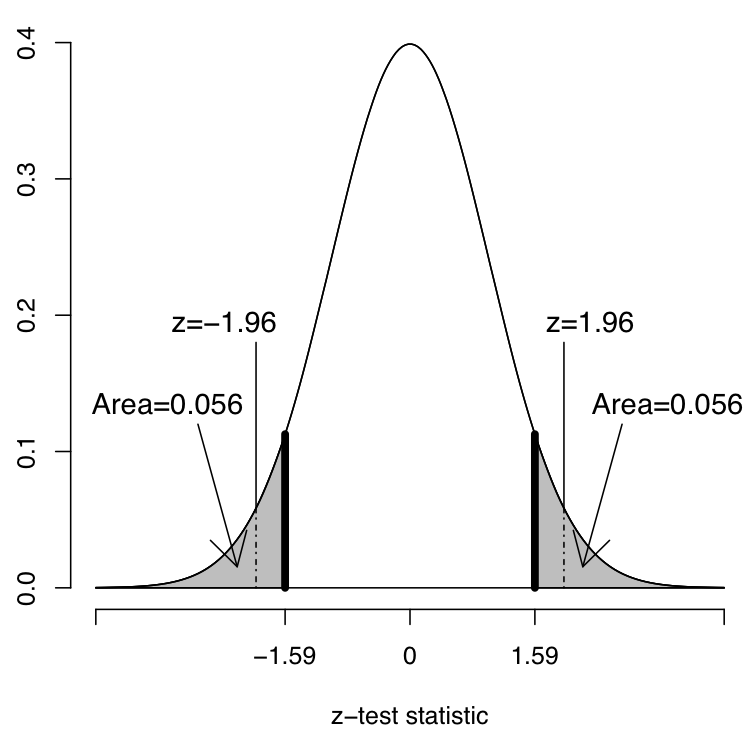
\includegraphics[width=10cm]{pval_zp}
%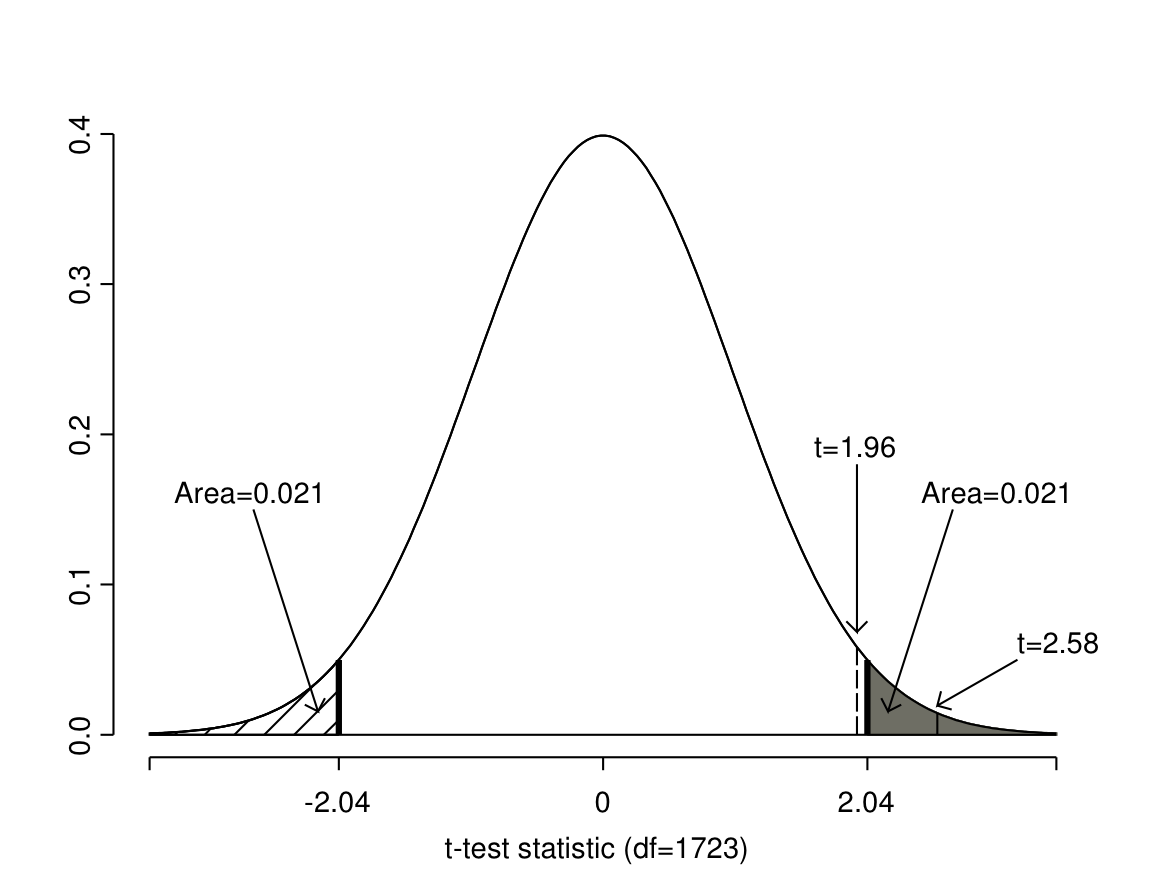
\includegraphics[width=13.5cm]{pvalsfat}
%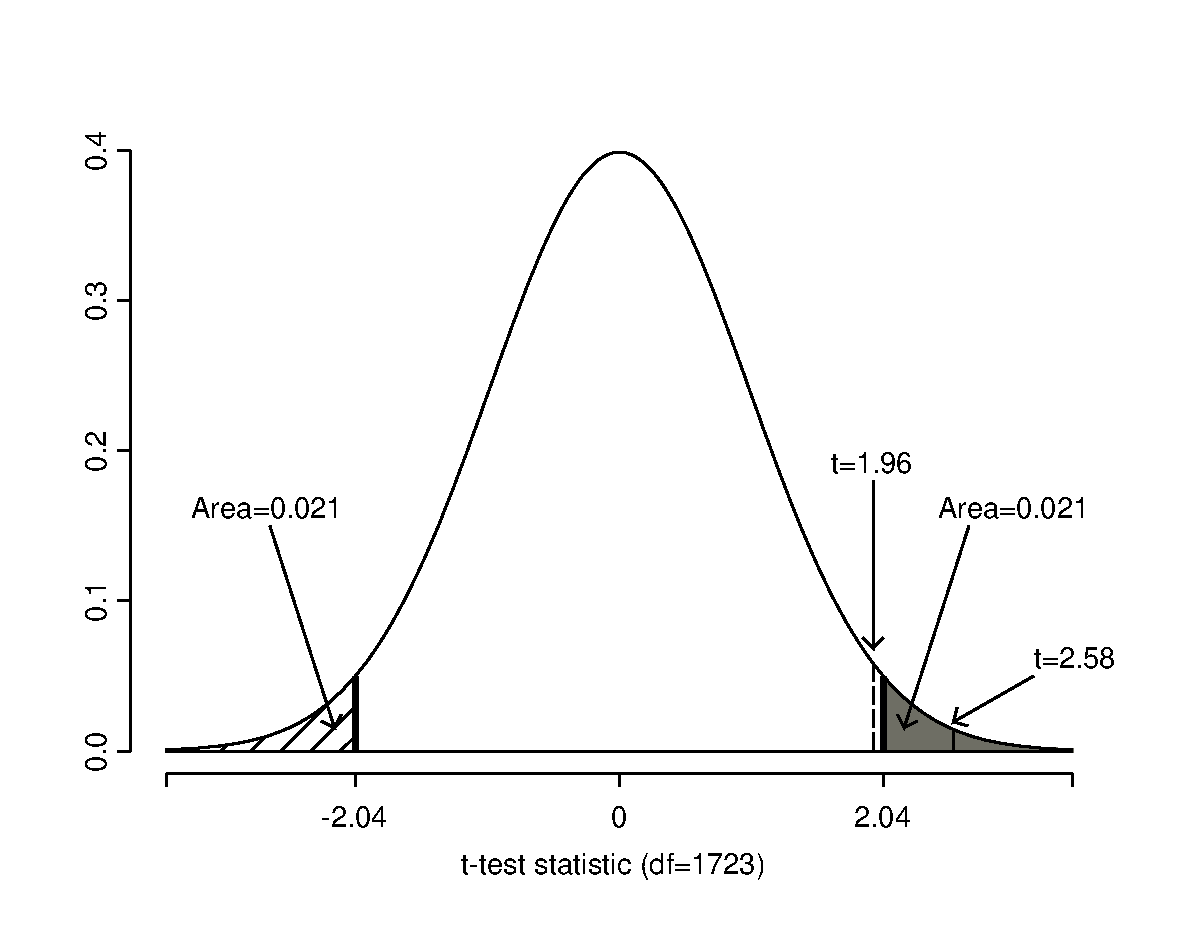
\epsfig{file=pvalsfat.eps, height=8.5cm}
\end{center}
\vspace*{-4ex}
\end{figure}

The $P$-value of the test is calculated from this distribution using the
general principles introduced in Section \ref{ss_tables_chi2test_Pval}.
In other words, the $P$-value is the probability that the test statistic
$z$ has a value that is as or more extreme than the value of $z$ in the
observed sample. Now, however, the details of this calculation depend
also on the alternative hypothesis, so some additional explanation is
needed.

Consider first the more common case of a two-sided alternative
hypothesis (\ref{Hatwo}), that $\Delta\ne 0$. As discussed in the
previous section, it is \emph{large} values of the test statistic which
indicate evidence against the null hypothesis, because a large $z$ is
obtained when the sample difference $\hat{\Delta}=\hat{\pi}-\pi_{0}$ is
very different from the zero difference claimed by the null hypothesis.
When the alternative is two-sided, ``large'' is taken to mean any value
of $z$ far from zero, i.e.\ either large positive or large negative
values, because both indicate that the sample difference is far from 0.
If $z$ is large and positive, $\hat{\Delta}$ is much \emph{larger} than
0. In example 5.1 this would indicate that a much larger proportion than
0.5 of the sample say they intend to vote Yes. If $z$ is
large and negative, $\hat{\Delta}$ is much \emph{smaller} than 0,
indicating a much smaller sample proportion than 0.5. Both of these
cases would count as evidence against $H_{0}$ when the alternative
hypothesis is two-sided.

The observed value of the $z$-test statistic in Example 5.1 was actually
$z=-1.59$. Evidence would thus be ``as strong'' against $H_{0}$ as the
observed $z$ if we obtained a $z$-test statistic of $-1.59$ or 1.59, the
value exactly as far from 0 as the observed $z$ but above rather than
below 0. Similarly, evidence against the null would be even stronger if
$z$ was further from zero than 1.59, i.e.\ larger than 1.59 or smaller
than $-1.59$. To obtain the $P$-value, we thus need to calculate the
probability of observing a $z$-test statistic which is at most $-1.59$
or at least 1.59 when the null hypothesis is true in the population. In
general, the $P$-value for testing the null hypothesis against a
two-sided alternative is the probability of obtaining a value at least
$z$ or at most $-z$ (when $z$ is positive, vice versa when it is
negative), where $z$ here denotes the value of the test statistic in the
sample. Such probabilities are calculated from the approximately
standard normal sampling distribution of the test statistic under
$H_{0}$.

This calculation of the $P$-value is illustrated graphically in Figure
\ref{f_pval_prob}. The curve in the plot is that of the standard normal
distribution. Two areas are shown in grey under the curve, one on each
tail of the distribution. The one on the left corresponds to values of
$-1.59$ and smaller, and the one on the right to values of 1.59 or
larger. Each of these areas is about 0.056, and the $P$-value for a test
against a two-sided alternative is their combined area, i.e.\
$P=0.056+0.056=0.112$. This means that even if the true population
proportion of Yes-voters was actually exactly 0.5, there would be a
probability of 0.112 of obtaining a test statistic as or more extreme
than the $z=-1.59$ that was actually observed in Example 5.1.

In example 5.2 the observed test statistic was $z=-16.71$. The
two-sided $P$-value is then the probability of values that are
at most $-16.71$ or at least 16.71. These areas are not shown in Figure
\ref{f_pval_prob} because they would not be visible in it. The horizontal
axis of the figures runs from $-4$ to $+4$, so $-16.71$ is clearly far
in the tail of the distribution and the corresponding probability is
very small; we would report it as $P<0.001$.

\label{p_onesided}
Consider now the case of a one-sided alternative hypothesis. For
example, in the referendum example we might have decided beforehand to
focus only on the possiblity that the proportion of people who intend to
vote Yes is smaller than 0.5, and hence consider the alternative
hypothesis that $\Delta<0$. Two situations might then arise. First,
suppose that the observed value of the sample difference is in the
direction indicated by the alternative hypothesis. This is the case in
the example, where the sample difference $\hat{\Delta}=-0.03$ is indeed
smaller than zero, and the test statistic $t=-1.59$ is negative. The
possible values of $z$ contributing to the $P$-value are then those of
$-1.59$ or smaller. Values of $1.59$ and larger are now not included,
because positive values of the test statistic (corresponding to sample
differences greater than 0) would not be regarded as evidence in favour
of the claim that $\Delta$ is smaller than 0. The $P$-value is thus only
the probability corresponding to the area on the left tail  of the curve
in Figure \ref{f_pval_prob}, and the corresponding area on the right
tail is not included. Since both areas have the same size, the one-sided
$P$-value is half the two-sided value, i.e.\ 0.056 instead of 0.112. In
general, the one-sided $P$-value for a $z$-test of a proportion and
other similar tests is always obtained by dividing the two-sided value
by 2, if the sample evidence is in the direction of the one-sided
alternative hypothesis.

The second case occurs when the sample difference is not in the
direction indicated by a one-sided alternative hypothesis. For example,
suppose that the sample proportion of Yes-voters had actually been 0.53,
i.e.\ 0.03 larger than 0.5, so that we had obtained $z=+1.59$ instead.
The possible values of the test statistic which contributed to the
$P$-value would then be $z=1.59$ and all smaller values. These are ``as
strong or stronger evidence against the null hypothesis and in the
direction of the alternative hypothesis'' as required by the definition
on page \pageref{p_pval_ref}, since they agree with the alternative
hypothesis (negative values of $z$) or at least disagree with it less
than the observed $z$ (positive values from 0 to 1.59). In Figure
\ref{f_pval_prob}, these values would correspond to the area under the
whole curve, apart from the region to the right of $1.59$ on the right
tail. Since the probability of the latter is 0.056 and the total
probability under the curve is 1, the required probability is
$P=1-0.0.56=0.944$. However, calculating the $P$-value so precisely is
hardly necessary in this case, as it is clearly going to be closer to 1
than to 0. The conclusion from such a large $P$-value will always be
that the null hypothesis should not be rejected. This is also
intuitively obvious, as a sample difference in the opposite direction
from the one claimed by the alternative hypothesis is clearly not to be
regarded as evidence in favour of that alternative hypothesis. In short,
if the sample difference is in a different direction than a one-sided
alternative hypothesis, the $P$-value can be reported simply as $P>0.5$
without further calculations.

If a statistical software package is used to carry out the
test, it will
also report the $P$-value and no further calculations are needed (except
dividing a two-sided $P$-value by 2, if a one-sided value is
needed and only a two-sided one is reported). However, since SPSS does
not currently provide a procedure for this test, and for exam purposes,
we will briefly outline how an approximate $P$-value is obtained using
critical values from a table. This is done in a very similar way as for
the $\chi^{2}$ test in Section \ref{ss_tables_chi2test_Pval}.

The first part of Table \ref{t_ttable} shows a table of critical values
for the standard normal distribution. These
values are also shown on page \pageref{s_disttables_t} at the end of
this course pack, on the last row of a larger table (the other parts of
this table will be explained later, in Section
\ref{ss_means_inference_variants}). A version of this
table is included in all introductory text books on statistics, although
its format may be slightly different in different books.

\begin{table}
\caption{A table of critical values for
the standard normal distribution. The upper part of the table shows
the critical values in one row, as in standard statistical tables
(see the last row of the table on page \pageref{s_disttables_t}). The
lower part of the table includes the same numbers rearranged
to show
critical values for conventional significance levels for one- and
two-sided tests.
}
\label{t_ttable}
\begin{center}
\begin{tabular}{|l|rrrrrrr|}\hline
& \multicolumn{7}{|c|}{Right-hand tail probability} \\ \cline{2-8}
& 0.100 & 0.050 & 0.025 & 0.01 & 0.005 & 0.001 & 0.0005 \\ \hline
Critical value &
1.282 & 1.645 & 1.960 & 2.326 & 2.576 & 3.090 & 3.291 \\
\hline
\end{tabular}

\vspace*{3ex}
\begin{tabular}{|l|rrrr|}\hline
& \multicolumn{4}{|c|}{Significance level} \\ \cline{2-5}
Alternative hypothesis & 0.10 & 0.05 & 0.01 & 0.001 \\ \hline
Two-sided & 1.65 & 1.96 & 2.58 & 3.29\\
One-sided & 1.28 & 1.65 & 2.33 & 3.09 \\ \hline
\end{tabular}
\end{center}
\end{table}

The columns of the first part of Table \ref{t_ttable} are labelled
``Right-hand tail probabilities'', with separate columns for some values
from 0.100 to 0.0005. This means that the probability that a value from
the standard normal distribution is at least as large as
the value given in a particular column is the
number given at the top of that column. For example, the value in the
column labelled ``0.025'' is 1.960, indicating that the probability of
obtaining a value equal to or greater than 1.960 from the standard normal
distribution is 0.025. Because the distribution is symmetric, the
probability of values of at most $-1.960$ is also 0.025, and the total
probability that a value is at least 1.960 units from zero is
$0.025+0.025=0.05$.

These values can be used to obtain bounds for $P$-values, expressed in
terms of conventional  significance levels of 0.10, 0.05, 0.01 and
0.001. The values at which these tail probabilities are obtained are the
corresponding critical values for the test statistic. They are shown in
the lower part of Table \ref{t_ttable}, slightly rearranged for clarity
of presentation and rounded to two decimal places (which is accurate
enough for practical purposes).
The basic idea of using the critical values is that if the observed
(absolute value of) the $z$-test statistic is \emph{larger} than a
critical value (for the required kind of alternative hypothesis) shown
in the lower part of Table \ref{t_ttable}, the $P$-value is
\emph{smaller} than the significance level corresponding to that
critical value.

The table shows only positive critical values. If the observed test
statistic is actually negative, its negative ($-$) sign is omitted and
the resulting positive value (i.e.\ the absolute value of the statistic)
is compared to the critical values. Note also that the critical value
for a given significance level depends on whether the alternative
hypothesis is two-sided or one-sided. In the one-sided case, the test
statistic is compared to the critical  values only if it is actually in
the direction of the alternative hypothesis; if not, we can simply
report $P>0.5$ as discussed above.

The $P$-value obtained from the table is reported as being smaller than
the smallest conventional significance level for which the corresponding
critical value is exceeded by the observed test statistic. For instance,
in the jury example 5.2 we have $z=-16.71$. Considering a two-sided
alternative hypothesis, 16.71 is larger than the critical values 1.65,
1.96, 2.58 and 3.29 for all the standard significance levels, so we can
report that $P<0.001$. For Example 5.1, in contrast, $z=-1.59$, the
absolute value of which is smaller than even the critical value 1.65 for
the 10\% significance level. For this example, we would report $P>0.1$.

The intuitive idea of the critical values and their connection to the
$P$-values is illustrated for Example 5.1 by Figure \ref{f_pval_prob} on
page \pageref{f_pval_prob}. Here the observed test statistic is
$t=-1.59$, so the two-sided $P$-value is the probability of values at
least 1.59 or at most $-1.59$, which correspond to the two gray areas in the
tails of the distribution. Also shown in the plot is one of the critical
values for two-sided tests, the 1.96 for significance level 0.05. By
definition of the critical values, the combined tail probability of
values at least 1.96 from 0, i.e.\ the probability of values at least
1.96 or at most $-1.96$, is 0.05. It is clear from the plot that since
1.59 is smaller than 1.96, these areas are smaller than the tail areas
corresponding to 1.59 and $-1.59$, and the combined area of the latter
must be more than 0.05, i.e.\ it must be that $P>0.05$. Similar argument
for the 10\% critical value of 1.65 shows that $P$ is here also larger
than 0.1.

\subsection{Conclusions from the test}
\label{ss_probs_test1sample_conclusions}

The general principles of drawing and stating conclusions from a
significance test have already been explained in Section
\ref{ss_tables_chi2test_conclusions}, so they need not be repeated here.
Considering two-sided alternative hypotheses, the conclusions in our
two examples are as follows:
\begin{itemize}
\item
In the referendum example 5.1, $P=0.112$ for the null hypothesis that
$\pi=0.5$ in the population of eligible voters. The null hypothesis is
not rejected at conventional levels of significance. There is not enough
evidence to conclude that the proportion of voters who definitely intend
to vote Yes differs from one half.
\item
In the jury example 5.2, $P<0.001$ for the null hypothesis that
$\pi=0.124$. The null hypothesis is thus overwhelmingly rejected at any
conventional level of significance. There is very strong evidence that
the probability of a black person being selected to the jury pool
differs from the proportion of blacks in the population of the county.
\end{itemize}

\subsection{Summary of the test}
\label{ss_probs_test1sample_summary}

As a summary, let us again repeat the main steps of the test described in this section
in a concise form, using the voting variable of
Example 5.1 for
illustration:
\begin{enumerate}
\item
Data: a sample of size $n=702$ of a dichotomous variable $Y$ with values
1 (Yes) and 0 (No or undecided), with the sample proportion
of ones $\hat{\pi}=0.47$.
\item
Assumptions: the observations are a random sample
from a population distribution with some
population proportion (probability) $\pi$, and the sample size $n$ is
large enough for the test to be valid
(for example, $n\ge 30$ when $\pi_{0}$ is between about 0.3 and 0.7, as it is here).
\item
Hypotheses: null hypothesis $H_{0}: \pi=\pi_{0}$ against the alternative
hypothesis $H_{a}: \pi\ne \pi_{0}$, where $\pi_{0}=0.5$.
\item
The test statistic: the $z$-statistic
\[
z=\frac{\hat{\pi}-\pi_{0}}{\sqrt{\pi_{0}(1-\pi_{0})/n}}=
\frac{0.47-0.50}{\sqrt{0.50\times(1-0.50)/702}}=-1.59.
\]
\item
The sampling distribution of the test statistic when $H_{0}$ is true: a
standard normal distribution.
\item
The $P$-value: the probability that a randomly selected value from the
the standard normal distribution is at most $-1.59$ or at least 1.59,
which is $P=0.112$.
\begin{itemize}
\item
If the precise $P$-value is not available,
we can observe that 1.59 is smaller than the
two-sided critical value 1.65 for the 10\% level of significance. Thus
it must be that $P>0.1$.
\end{itemize}
\item
Conclusion: The null hypothesis is not rejected ($P=0.112$).
There is not enough evidence to conclude that the proportion of eligible
voters who definitely intend to vote Yes differs from one half. Based on this
opinion poll, the referendum remains too close to
call.
\end{enumerate}

\section{Confidence interval for a single proportion}
\label{s_probs_1sampleci}

\subsection{Introduction}
\label{s_probs_1sampleci_intro}

A significance test assesses whether it is plausible, given the evidence
in the observed data, that a population parameter or parameters have a
specific set of values claimed by the null hypothesis. For example, in Section
\ref{s_probs_test1sample} we asked such a question about the probability
parameter of a binary variable in a single population.

In many ways a
more natural approach would be try to identify all of those values of
a parameter which \emph{are} plausible given the data. This leads to a form
of statistical inference known as \textbf{interval estimation}, which
aims to present not only a single best guess (i.e.\ a point estimate) of
a population parameter, but also a range of plausible values (an
\textbf{interval estimate}) for it. Such an interval is known as a
\textbf{confidence interval}. This section introduces the idea of
confidence intervals, and shows how to construct them for a population
probability. In later sections, the same principles will be used to
calculate confidence intervals for other kinds of population parameters.

Interval estimation is an  often underused part of
statistical inference, while significance testing is arguably overused
or at least often misused. In most contexts it would be useful to report
confidence intervals in addition to, or instead of, results of
significance tests. This is not done often enough in
research publications in the social sciences.

\subsection{Calculation of the interval}
\label{s_probs_1sampleci_calc}

Our aim is again to draw inference on the difference
$\Delta=\pi-\pi_{0}$ or, equivalently, the population probability $\pi$.
The point estimate of $\Delta$ is $\hat{\Delta}=\hat{\pi}-\pi_{0}$ where
$\hat{\pi}$ is the sample proportion corresponding to $\pi$. Suppose
that the conditions on the sample size $n$ that were discussed in
Section \ref{ss_probs_test1sample_samplingd} are again satisfied.

Consider now Figure \ref{f_pval_prob} on \pageref{f_pval_prob}. One of
the results illustrated by it is that if $\pi_{0}$ is the true value of
of the population probability $\pi$, so that $\Delta=\pi-\pi_{0}=0$, there is a
probability of 0.95 that for a randomly drawn sample from the population
the $z$-test statistic $z=\hat{\Delta}/\hat{\sigma}_{\hat{\Delta}}$ is
between $-1.96$ and $+1.96$. This also implies that the probability is
0.95 that in such a sample the observed value of $\hat{\Delta}$ will be
between $\Delta-1.96\,\hat{\sigma}_{\hat{\Delta}}$ and
$\Delta+1.96\,\hat{\sigma}_{\hat{\Delta}}$. Furthermore, it is clear
from the figure that all of the values within this interval are more
likely to occur than any of the values outside the interval (i.e.\ those
in the two tails of the sampling distribution). The interval thus seems
like a sensible summary of the ``most likely'' values that the estimate
$\hat{\Delta}$ may have in random samples.

A confidence interval essentially turns this around, into a statement
about the unknown true value of $\Delta$ in the population, even in
cases where $\Delta$ is not 0.
This is done by substituting $\hat{\Delta}$ for $\Delta$
above, to create the interval
\begin{equation}
\text{from  }\hspace*{1em}
\hat{\Delta} -1.96\times \hat{\sigma}_{\hat{\Delta}}
\hspace*{1em}\text{  to  }\hspace*{1em}
\hat{\Delta}
+1.96\times \hat{\sigma}_{\hat{\Delta}}.
\label{cim0}
\end{equation}
This is the \textbf{95 \% confidence interval} for the population
difference $\Delta$. It is
usually written more concisely as
\begin{equation}
\hat{\Delta}
\pm 1.96\, \hat{\sigma}_{\hat{\Delta}}
\label{cim1}
\end{equation}
where the ``plusminus'' symbol $\pm$ indicates that we calculate the two
endpoints of the interval as in (\ref{cim0}), one below and one above
$\hat{\Delta}$.

Expression (\ref{cim1}) is general in the sense that many different
quantities can take the role of $\Delta$ in it. Here we consider for now
the case of $\Delta=\pi-\pi_{0}$. The estimated standard error
$\hat{\sigma}_{\hat{\Delta}}$ is analogous to
(\ref{seDhatp}) used for the $z$-test, but not the same.
This is because the confidence interval
is not calculated under the null hypothesis $H_{0}:\; \pi=\pi_{0}$, so
we cannot use $\pi_{0}$ for $\pi$ in the standard error. Instead, $\pi$
is estimated by the sample proportion $\hat{\pi}$, giving the estimated
standard error
\begin{equation}
\hat{\sigma}_{\hat{\Delta}} = \sqrt{
\frac{\hat{\pi}(1-\hat{\pi})}{n}
}
\label{sephat2}
\end{equation}
and thus the 95\% confidence interval
\[
(\hat{\pi}-\pi_{0}) \pm 1.96 \;
\sqrt{
\frac{\hat{\pi}(1-\hat{\pi})}{n}}
\]
for $\Delta=\pi-\pi_{0}$. Alternatively, a confidence interval for
$\pi$ itself is given by
\begin{equation}
\hat{\pi} \pm 1.96 \;
\sqrt{
\frac{\hat{\pi}(1-\hat{\pi})}{n}}.
\label{cip2}
\end{equation}
This is typically the most useful interval for use in practice.
For instance, in the referendum example 5.1 this
gives a 95\% confidence interval of
\[
0.470\pm 1.96\times \sqrt{\frac{0.470\times(1-0.470)}{702}}
=0.470\pm 0.0369=(0.433, 0.507)
\]
for the proportion of definite Yes-voters in the population. Similarly,
in Example 5.2 the 95\% confidence interval for the probability of a
black person being selected for the jury pool is (0.040, 0.052). These
intervals are also shown in Table \ref{t_probex}.

\subsection{Interpretation of confidence intervals}
\label{s_probs_1sampleci_int}

As with the $P$-value of a significance test, the precise
interpretation of a confidence interval refers to probabilities
calculated from a sampling distribution, i.e.\ probabilities evaluated
from a hypothetical exercise of repeated sampling:
\begin{itemize}
\item
If we obtained many samples from the population and calculated the
confidence interval for each such sample using the formula (\ref{cip2}),
approximately 95\% of these intervals would contain the true
value of the population proportion $\pi$.
\end{itemize}
This is undeniably convoluted, even more so than the precise
interpretation of a $P$-value. In practise a confidence
interval would not usually be described in exactly these words. Instead, a
research report might, for example, write that (in the
referendum example)
``the 95 \% confidence interval for the proportion of eligible voters in
the population who definitely intend to vote Yes is (0.433, 0.507)'',
or that ``we are 95 \%
confident that the proportion of eligible voters in the population who
definitely intend to vote Yes is between 43.3\% and 50.7\%''.
Such a statement in effect assumes that the readers will be
familiar enough with the idea of confidence intervals to understand the
claim. It is nevertheless useful to be aware of the more
careful interpretation of a confidence interval, if only to avoid
misunderstandings. The most common error is to claim that
``there is a 95\% probability that the
proportion in the population is between 0.433 and 0.507''.
Although the difference to the interpretation given above
may seem small, the latter statement is not really true, or strictly
speaking even meaningful, in the statistical framework considered here.

In place of the 1.96 in (\ref{cim1}), we may also use other numbers.
To allow for this in the notation, we can also write
\begin{equation}
\hat{\Delta} \pm z_{\alpha/2}\; \hat{\sigma}_{\hat{\Delta}}.
\label{ci_D_gen}
\end{equation}
where the multiplier $z_{\alpha/2}$ is a number which depends
on two things. One of them is the sampling distribution of
$\hat{\Delta}$, which is here assumed to be the normal distribution
(another possibility is discussed in Section
\ref{ss_means_inference_variants}). The second is
the \textbf{confidence level} which we have chosen for the confidence
interval. For example, the probability of 0.95 in the interpretation of
a 95\% confidence interval discussed above is the confidence level of
that interval. Conventionally the 0.95 level is most commonly used,
while other standard choices are 0.90 and 0.99, i.e.\ 90\% and 99\%
confidence intervals.

In the symbol $z_{\alpha/2}$, $\alpha$ is a number such that $1-\alpha$
equals the required confidence level. In other words, $\alpha=0.1$,
0.05, and 0.01 for confidence levels of $1-\alpha=0.90$, 0.95 and 0.99
respectively. The values that are required for the conventional levels
are $z_{0.10/2}=z_{0.05}=1.64$, $z_{0.05/2}=z_{0.025}=1.96$, and
$z_{0.01/2}=z_{0.005}=2.58$, which correspond to intervals at the
confidence levels of 90\%, 95\% and 99\% respectively. These values are
also shown in Table \ref{t_ciq}.

\begin{table}
\caption{Multipliers $z_{\alpha/2}$ used to obtain confidence intervals
based on the normal distribution, for three standard confidence
levels. These values are substituted for $z_{\alpha/2}$ in formula
(\ref{ci_D_gen}) to obtain the confidence interval.}
\label{t_ciq}
\begin{center}
\begin{tabular}{|l|rrr|}\hline
& \multicolumn{3}{|c|}{Confidence level} \\
& 90\% & 95\% & 99\% \\ \hline
Multiplier $z_{\alpha/2}$ & 1.64 & 1.96 & 2.58 \\
\hline
\end{tabular}
\end{center}
\end{table}

A confidence interval contains, loosely speaking, those numbers which
are considered plausible values for the unknown population difference
$\Delta$ in
the light of the evidence in the data. The \emph{width} of the interval
thus reflects our uncertainty about the exact value of $\Delta$, which
in turn is related to the amount of information the data provide about
$\Delta$. If the interval is wide, many values are consistent with the
observed data, so there is still a large amount of uncertainty; if the
interval is narrow, we have much information about $\Delta$ and thus little
uncertainty. Another way of stating this is that when the confidence
interval is narrow, estimates of $\Delta$ are very \emph{precise}.

The width of the interval (\ref{ci_D_gen}) is
$2\times z_{\alpha/2}\times \hat{\sigma}_{\hat{\Delta}}$.
This depends on
\begin{itemize}
\item
The confidence level: the higher the level, the wider the interval. Thus
a 99\% confidence interval is always wider than a 95\% interval for the
same data, and wider still than a 90\% interval. This is logically
inevitable: if we want to state with high level of confidence that a
parameter is within a certain interval, we must allow the
interval to contain a wide range of values. It also explains why we do
not consider a 100\% confidence interval: this would contain all
possible values of $\Delta$ and exclude none, making no use of
the data at all. Instead, we aim for a high but not perfect level of
confidence, obtaining an interval which contains some but not all
possible values, for the price of a small chance of incorrect conclusions.
\item
The standard error $\hat{\sigma}_{\hat{\Delta}}$, which in the
case of a single proportion is (\ref{sephat2}).
This in turn depends on
\begin{itemize}
\item
the sample size $n$: the larger this is, the narrower the interval.
Increasing the sample size thus results (other things being
equal) in reduced uncertainty and higher precision.
\item
the true population proportion $\pi$:
the closer this is to 0.5, the wider the interval.
Unlike the sample size, this determinant
of the estimation uncertainty is not in our control.
\end{itemize}
\end{itemize}
Opinion polls of the kind illustrated by the referendum example are probably
where non-academic audiences are most likely to encounter confidence
intervals, although not under that label. Media reports of such polls
typically include a \emph{margin of error} for the results. For example,
in the referendum example it might be reported that
47\% of the respondents said that they would definitely vote Yes, and
that ``the study has a margin of error of plus or
minus four percentage points''.
In most cases the phrase ``margin of
error'' refers to a 95\% confidence interval. Unless otherwise
mentioned, we can thus take a statement like the one above to mean that
the 95\% confidence interval for the proportion of interest is
approximately $47\pm 4$
percentage points. For a realistic interpretation of the implications of
the results, the width of this interval is at least as important as the
point estimate of the proportion. This is often neglected in media
reports of opinion polls, where the point estimate tends to be headline
news, while the margin of error is typically mentioned only in passing
or omitted altogether.

\subsection{Confidence intervals vs.\ significance tests}
\label{ss-means-ci-vstests}

There are some obvious similarities between the conclusions from significance tests and
confidence intervals. For example, a $z$-test in the referendum example
5.1 showed that the null hypothesis that the population proportion
$\pi$ was 0.5 was not rejected ($P=0.112$).
Thus 0.5 is a plausible value for $\pi$ in light of the observed
data. The 95\% confidence interval for $\pi$ showed that, at this
level of confidence, plausible values for $\pi$ are those between
0.433 and 0.507. In particular, these include 0.5, so the confidence
interval also indicates that a proportion of 0.5 is plausible.
This connection between the test and the confidence interval is in fact
exact:
\begin{itemize}
\item
If the hypothesis $H_{0}: \Delta=0$ about a population quantity
$\Delta$
is rejected at the 5\% level of significance using the $z$-test
against a \emph{two-sided} alternative
hypothesis, the 95 \% confidence interval for $\Delta$
will not contain
0, and vice versa. Similarly, if $H_{0}$ is not rejected, the
confidence interval will contain 0, and vice versa.
\end{itemize}
The same is true for other matching pairs of levels of
significance and confidence, e.g.\ for a test with a 1\% level of
significance and a 99\% (i.e.\ (100-1)\%) confidence interval. In short,
the significance test and the confidence interval will in these cases
always give the same answer about whether or not a parameter value is
plausible (consistent with the data) at a given level of
significance/confidence.

These pairs of a test and an interval are exactly
comparable in that they concern the same population parameter, estimate
all parameters in the same way, use the same sampling distribution for
inference, and use the same level of significance/confidence. Not all
tests and confidence intervals have exact pairs in this way. Also, some
tests are for hypotheses about more than one parameter at once, so there
is no corresponding single confidence interval. Nevertheless, the
connection stated above is useful for understanding the ideas of both
tests and confidence intervals.

\label{p_civstest}
These results also illustrate how confidence intervals are inherently
more informative than significance tests. For instance, in the jury
example 5.2, both the test and the confidence interval
agree on the implausibility of the claim that the population probability of being selected
to the jury panel is the same as the proportion (0.124) of black people
in the population, since the claim that $\pi=0.124$ is rejected
by the test (with $P<0.001$) and outside the interval $(0.040; 0.052)$.
Unlike the test, however, the confidence
interval summarizes the plausibility of \emph{all} possible values of
$\pi$ and not just $\pi_{0}=0.124$. One way to describe this is to consider what
would have happened if we had carried out a series of significance tests
of null hypotheses of the form $H_{0}: \pi=\pi_{0}$ for a range of
values of $\pi_{0}$.
The confidence interval
contains all those values $\pi_{0}$ which would not have been
rejected by the test, while all the values outside the interval would
have been rejected. Here $H_{0}: \pi=\pi_{0}$ would thus not have
been rejected at the 5\% level if $\pi_{0}$ had been between 0.040 and
0.052, and rejected otherwise. This, of course, is not how significance
tests are actually conducted, but it provides a useful additional
interpretation of confidence intervals.

A confidence interval is particularly useful when the parameter of
interest is measured in familiar units, such as the proportions
considered so far. We may then try to judge, in substantive terms,
how wide the interval is and how far it is from particular values of
interest. In the jury example the 95\% confidence interval ranges from
4.0\% to 5.2\%, which suggests that the population probability is
estimated fairly precisely by this survey. The interval also reveals
that even its upper bound is less than half of the figure of
12.4\% which would correspond to proportional representation of blacks
in the jury pool, a  result which suggests quite substantial
underrepresentation in the pool.

\section{Inference for comparing two proportions}
\label{s_probs_2samples}

In Examples 5.3 and 5.4, the aim is to compare the
proportion of a dichotomous response variable $Y$ between two groups of a
dichotomous explanatory variable $X$:
\begin{itemize}
\item
Example 5.3: compare the proportion of polio cases among the
unvaccinated ($\pi_{1}$) and vaccinated ($\pi_{2}$) children.
\item
Example 5.4: compare
the proportion of
optimistic responses to a negative ($\pi_{1}$)
vs.\ positive wording of the question ($\pi_{2}$).
\end{itemize}
The quantity of interest is then the population difference
\begin{equation}
\Delta=\pi_{2}-\pi_{1}.
\label{Dp2sample}
\end{equation}
For a significance test of this, the null hypothesis will again be $H_{0}:\; \Delta=0$,
which is in this case equivalent to the hypothesis of equal proportions
\begin{equation}
H_{0}:\; \pi_{1} = \pi_{2}.
\label{H0pD}
\end{equation}
The null hypothesis thus claims that there is no association between
the group variable $X$ and the dichotomous response variable $Y$,
while the alternative hypothesis
(e.g.\  the two-sided one
$H_{a}:\; \pi_{1}\ne \pi_{2}$, i.e.\ $H_{a}:\; \Delta\ne
0$) implies that there is an association.

The obvious estimates of $\pi_{1}$ and $\pi_{2}$ are
the corresponding sample proportions $\hat{\pi}_{1}$ and
$\hat{\pi}_{2}$, calculated from samples of sizes $n_{1}$ and $n_{2}$
respectively, and the estimate of $\Delta$ is then
\begin{equation}
\hat{\Delta}=\hat{\pi}_{2} - \hat{\pi}_{1}.
\label{Dhatpi}
\end{equation}
This gives $\hat{\Delta}=0.000284-0.000706=-0.000422$ in Example 5.3 and
$\hat{\Delta}=0.364-0.279=0.085$ in Example 5.4.
In the samples, the proportion of
polio cases is thus lower in the vaccinated group, and the proportion of
optimistic answers is higher in response to a positively worded
question. Note also that although the inference discussed below focuses
on the difference of the proportions,
for purely descriptive purposes
we might prefer to use some other statistic,
such as the ratio of the proportions.
For example, the difference of 0.000422 in polio
incidence between vaccine and control groups may seem small, because the
proportions in both groups are small. A better idea of the the magnitude
of the contrast is given by their ratio of $0.000706/0.000284=2.49$
(this is known as the \emph{risk ratio}). In other words, the rate of
polio infection in the unvaccinated group was two and a half times the
rate in the vaccinated group.

\label{p2pthumb}
The tests and confidence intervals discussed below are again based on
the assumption that the relevant sampling distributions are
approximately normal, which is true when the sample sizes $n_{1}$ and
$n_{2}$ are large enough. The conditions for this are not very
demanding: one rule of thumb states that the methods described in this
section are reasonably valid if in both groups the number of
observations with $Y$ having the value 1, and of ones with the value 0,
are both more than 5. This condition is satisfied in both of the
examples considered here.

The validity of the test, as well as the amount of information the data
provide about $\pi_{1}$ and $\pi_{2}$ in general, thus depends not just
on the overall sample sizes but on having enough observations of both
values of $Y$. The critical quantity is then the number of observations
in the rarer category of $Y$. In Example 5.3 this means the numbers of
children diagnosed with polio, because the probability of polio was
 low in the study population. The numbers of eventual polio
cases were 142 and 57 in the control and treatment groups respectively,
so the rule of thumb stated above was satisfied. With such low
probabilities of polio incidence, sufficient numbers of cases were
achieved only by making the overall sample sizes $n_{1}$ and $n_{2}$
large enough. That is why the trial had to be very large, involving
hundreds of thousands of participants.

The standard error of $\hat{\Delta}$ is
\begin{equation}
\sigma_{\hat{\Delta}} =
\sqrt{
\frac{\pi_{2}(1-\pi_{2})}{n_{2}}
+\frac{\pi_{1}(1-\pi_{1})}{n_{1}}
}.
\label{sigmaDpi}
\end{equation}
As in the one-sample case above, the best way to estimate this
is different for a significance test than for a confidence interval.
For a test, the standard error can be estimated under assumption that
the null
hypothesis (\ref{H0pD}) is true,
in which case the population proportion is the
same in both groups. A good estimate of this common proportion, denoted
below by $\hat{\pi}$,
is the proportion of observations
with value 1 for $Y$ in the total sample of $n_{1}+n_{2}$ observations,
pooling observations from both groups together; expressed in terms of the
group-specific estimates, this is
\begin{equation}
\hat{\pi} = \frac{n_{1}\hat{\pi}_{1}+n_{2}\hat{\pi}_{2}}{n_{1}+n_{2}}.
\label{phat2sample}
\end{equation}
Using this for both
$\pi_{1}$ and $\pi_{2}$ in (\ref{sigmaDpi}) gives the
estimated standard error
\begin{equation}
\hat{\sigma}_{\hat{\Delta}}=
\sqrt{
\hat{\pi}(1-\hat{\pi}) \; \left(
\frac{1}{n_{2}}+
\frac{1}{n_{1}}
\right),
}
\label{seDpi}
\end{equation}
and using (\ref{Dhatpi}) and (\ref{seDpi}) in the general formula
(\ref{ttest_gen}) gives the \textbf{two-sample $z$-test statistic for
proportions}
\begin{equation}
z=
\frac{\hat{\pi}_{2}-\hat{\pi}_{1}}
{\sqrt{\hat{\pi}(1-\hat{\pi})(1/n_{2}+1/n_{1})}}
\label{ztestDpi}
\end{equation}
where $\hat{\pi}$ is given by (\ref{phat2sample}). When the null
hypothesis is true, the sampling distribution of this test statistic is
approximately standard normal when the sample sizes are large enough.

For a confidence interval, the calculation of the estimated standard error cannot
assume that (\ref{H0pD}) is true. Instead, we use
the estimate
\begin{equation}
\hat{\sigma}_{\hat{\Delta}} =
\sqrt{
\frac{\hat{\pi}_{2}(1-\hat{\pi}_{2})}{n_{2}} +
\frac{\hat{\pi}_{1}(1-\hat{\pi}_{1})}{n_{1}}
}
\label{seDpi2}
\end{equation}
and, substituting this to the general formula (\ref{ci_D_gen}), we get
\begin{equation}
(\hat{\pi}_{2}-\hat{\pi}_{1}) \pm z_{\alpha/2} \;
\sqrt{
\frac{\hat{\pi}_{2}(1-\hat{\pi}_{2})}{n_{2}} +
\frac{\hat{\pi}_{1}(1-\hat{\pi}_{1})}{n_{1}}
}
\label{ciDpi}
\end{equation}
as the
confidence interval
for $\Delta=\pi_{2}-\pi_{1}$, with confidence level $1-\alpha$.

For an illustration of the calculations, consider Example 5.4. Denoting
the group of respondents answering the negatively worded question by 1
and those with the positive question by 2, the basic quantities are
$n_{1}=921$, $\hat{\pi}_{1}=0.279$, $n_{2}=929$ and
$\hat{\pi}_{2}=0.364$. The estimated difference in the proportions of
respondents giving an optimistic answer is thus
\[
\hat{\Delta} = \hat{\pi}_{2}-\hat{\pi}_{1} = 0.364-0.279 = 0.085.
\]
For a significance test, the estimated standard error of $\hat{\Delta}$
uses the pooled estimate (\ref{phat2sample}) of the population
proportion, which is given by
\[
\hat{\pi} = \frac{921\times 0.279+929\times 0.364}{921+929}=
\frac{257+338}{921+929} = 0.322.
\]
The standard error from (\ref{seDpi}) is then
\[
\hat{\sigma}_{\hat{\Delta}}
=
\sqrt{
0.322\times(1-0.322) \times \left(
\frac{1}{929}+
\frac{1}{921}
\right)
}
=
\sqrt{
\frac{0.2182}{462.5}
}=0.0217,
\]
and the test statistic (\ref{ztestDpi}) is
\[
z=\frac{0.085}{0.0217}=3.92.
\]
For the confidence interval, the standard error of $\hat{\Delta}$
is estimated from (\ref{seDpi2}) as
\begin{eqnarray*}
\hat{\sigma}_{\hat{\Delta}} &=&
\sqrt{
\frac{0.364\times (1-0.364)}{929} +
\frac{0.279\times (1-0.279)}{921}
} \\
&=&
\sqrt{
\frac{0.2315}{929}
+\frac{0.2012}{921}
}=0.0216
\end{eqnarray*}
and a 95\%  confidence interval from (\ref{ciDpi}) is
\[
0.085 \pm 1.96 \times 0.0216 = 0.085\pm 0.042 = (0.043; 0.127).
\]
The $P$-value for the test statistic is clearly very low (in fact about
$0.00009$), so the null hypothesis of equal proportions is convincingly
rejected. There is very strong evidence that the probability that a
respondent will give an answer indicating optimism for the future is
different for the two differently worded questions. The confidence
interval indicates that we are 95\% confident that the proportion of
optimistic answers is between 4.3 and 12.7 percentage points higher when
the question is worded positively than when it is worded negatively.
This suggests quite a substantial acquiescence bias arising from
changing just one word in the survey question, as described in the
introduction to Example 5.4 at the beginning of this chapter.

In Example 5.3, the estimated difference
is $\hat{\Delta}=-0.000422$
(see Table
\ref{t_probex} on page \pageref{t_probex}),
i.e.\ 422 fewer
polio cases per million children in the vaccinated group
than in the unvaccinated group.
Similar calculations as above show that
the value of the test statistic is $z=-6.01$, so the
$P$-value is again very small (in fact about 0.000000001) and the null
hypothesis of equal probabilities is strongly rejected. There is thus
overwhelming evidence that the proportion of polio cases was different
among the vaccinated children than among the
unvaccinated ones.
The 95\% confidence interval for the difference
shows
that we are 95\% confident that this difference was a reduction of
between 284 and 560 polio cases per million children\footnote{Note that
incidence was not zero even in the vaccinated group, because the Salk
vaccine --- like most vaccines --- is not 100\% effective. Despite this,
it is possible for a broad enough vaccination programme to eliminate a
disease completely, by depriving it the chance to spread and
conferring so-called herd immunity for the whole
population. Conversely, if vaccination rates drop too low, herd immunity
is removed and the disease may reappear at a higher rate than implied by
the reduction in vaccination alone.}.
This was acknowledged as a convincing demonstration that the
Salk vaccine worked (see Figure \ref{f_nytimes}), and it (and later other types of polio vaccination)
was soon put to widespread use. The resulting dramatic decline in the
incidence of polio is one of the great success stories of modern
medicine. Compared to the 199 children with polio in 1954 among the less
than half a million participants of the vaccine trial alone, in 2014
there were 414 confirmed cases of polio in the whole world (see
\texttt{www.polioeradication.org/Dataandmonitoring/Poliothisweek.aspx}). There is hope that
that number will reach 0 in a not-too-distant future, so that the once
devastating disease will one day be entirely eradicated.

\begin{figure}
\caption{Public reaction to statistical inference.}
\label{f_nytimes}
\vspace*{4ex}
%
\includegraphics[angle=90, width=150mm]{salk_nytimes}

\includegraphics[width=150mm]{salk_nytimes}
\end{figure}
